\documentclass[12pt]{article}
\usepackage{amsmath}
\usepackage{amsfonts}
\usepackage{graphicx}
\usepackage{booktabs}
\usepackage{geometry}
\usepackage[numbers]{natbib}
\geometry{a4paper, margin=1in}

\begin{document}


% Introducing the ResNet architecture
\section{Residual Network (ResNet)}\label{sec:intro}
ResNet (or residual network) is a type of deep neural network that is able to perform very well, of with the vanishing gradient as depths grows. It applies residual blocks that have 3 convolutional blocks using different kernel size through shortcut connection that adds initial input to a block output. The ResNet as described in this work consists of three blocks and then is connected to a global average pooling layer and a fully connected layer for the final output.~\cite{chen2023}

% Describing the residual block and equations
\subsection{Residual Block}\label{subsec:resblock}
Each residual block uses 1 x 1 convolutions to create three convolutional blocks which are set up as follows:
\begin{align}
h_1 &= \text{ReLU}(\text{BN}(\text{Conv1d}(x))), \label{eq:h1} \\
h_2 &= \text{ReLU}(\text{BN}(\text{Conv1d}(h_1))), \label{eq:h2} \\
h_3 &= \text{BN}(\text{Conv1d}(h_2)). \label{eq:h3}
\end{align}
After computing \(h3\), the value is relayed to a linear unit. Output of the residual block is then calculated by \(x\) plus relaying \(h3\) while applying the relayed value on a linear unit:
\begin{align}
y &= h_3 + x, \label{eq:y} \\
\hat{h} &= \text{ReLU}(y). \label{eq:hhat}
\end{align}
The convolutional blocks use kernel sizes of 7, 5 and 3. The three residual blocks will have the filter count set to \( k_i = \{64, 128, 128\} \).

% Describing the overall ResNet structure
\subsection{ResNet Structure}\label{subsec:resnet}
The design layout of the ResNet model is as follows:
\[
\text{ResNet} = [\text{ResBlock1}, \text{ResBlock2}, \text{ResBlock3}, \text{GlobalAvgPooling}, \text{FC}].
\]
The model receives input data and computes it through the three residual blocks, then bounds global average pooling to spatial dimensionality reduction, then ultimately produces the output through a fully connected layer detached from the pooling operation.

\section{ResNetLSTM Model}\label{sec:resnetlstm}
The architecture of ResNet-LSTM includes ResNet for spatial feature extraction and LSTM for time-series modeling. We adopt ResNet based on ResNet18 to extract features by convolution processes along with residual blocks, which provide a feature tensor as input to the LSTM. The LSTM component incorporates temporal dependencies using 2 layers with 1024 and 256 units each. They utilized dropout to prevent overfitting as well as 2 dense layers for prediction which consisted of 64 and 1 neurons respectively.[1]. In the implemented model, an LSTM layer with 50 units is added to process the transposed ResNet output:
\begin{equation}
x_{\text{lstm}} = x.\text{transpose}(1, 2), \label{eq:transpose}
\end{equation}
followed by:
\begin{equation}
x_{\text{lstm}}, (h_n, c_n) = \text{LSTM}(x_{\text{lstm}}). \label{eq:lstm}
\end{equation}
The final time step output is selected:
\begin{equation}
x_{\text{final}} = x_{\text{lstm}}[:, -1, :]. \label{eq:final}
\end{equation}
The prediction is produced through the application of a fully connected (FC) layer:
\begin{equation}
y = \text{FC}(x_{\text{final}}). \label{eq:output}
\end{equation}
The total architecture is:
\[
\text{ResNetLSTM} = [\text{ResBlock1}, \text{ResBlock2}, \text{ResBlock3}, \text{LSTM}, \text{FC}].
\]
Model training was done using the Adam optimizer with a learning rate set at 0.001, mean squared error (MSE) loss, a batch size of 64, and 100 epochs.

\section{Experimental Results}
The evaluation metrics are calculated by measuring errors, such as Mean Absolute Error (MAE), Mean Absolute Percentage Error (MAPE), Mean Absolute Scaled Error (MASE), Mean Squared Error (MSE), and Root of Mean Squared Error (RMSE,).
\[
\text{MAE} = \frac{1}{n} \sum_{i=1}^n |y_i - \hat{y}_i|
\]
\[
\text{MAPE} = \frac{1}{n} \sum_{i=1}^n \left| \frac{y_i - \hat{y}_i}{y_i} \right| \times 100
\]
\[
\text{MASE} = \frac{1}{n} \sum_{i=1}^n \frac{|y_i - \hat{y}_i|}{\frac{1}{m-1} \sum_{j=1}^{m-1} |y_{j+1}^{\text{train}} - y_j^{\text{train}}|}
\]
\[
\text{MSE} = \frac{1}{n} \sum_{i=1}^n (y_i - \hat{y}_i)^2
\]
\[
\text{RMSE} = \sqrt{\frac{1}{n} \sum_{i=1}^n (y_i - \hat{y}_i)^2}
\]
where \( y_i \) is the actual price, \( \hat{y}_i \) is the predicted price, \( n \) is the number of predictions, and \( y^{\text{train}} \) is the training data.

The results are summarized in Table~\ref{tab:results}.

\begin{table}[ht]
\centering
\caption{Forecasting performance of ResNet and ResNetLSTM on the test set.}
\label{tab:results}
\begin{tabular}{lccccc}
\toprule
Model & MAE & MAPE (\%) & MASE & MSE & RMSE \\
\midrule
ResNet & 24.8383 & 8.7462 & 2651.4954 & 1253.6210 & 35.4065 \\
ResNetLSTM & 23.3139 & 7.7512 & 2488.7656 & 1254.4014 & 35.4175 \\
\bottomrule
\end{tabular}
\end{table}

% \section{Visualization}
% The forecasting results are visualized using Matplotlib, plotting actual and predicted ``Close'' prices in a 12$\times$6-inch figure titled ``Predict 90 Days Next''. The plot includes:

% \begin{itemize}
%     \item Training data: Inverse-transformed ``Close'' prices for the training set.
%     \item Testing data: Inverse-transformed ``Close'' prices for the testing set.
%     \item Predictions: Test set predictions (\texttt{test\_predict}) and forecasts for 30, 60, and 90 days (\texttt{lst\_output\_30}, \texttt{lst\_output\_60}, \texttt{lst\_output\_90}).
% \end{itemize}

% The plotting indices are:
% \begin{align}
% \text{train\_data\_index} &= [0, \text{train\_size}) \\
% \text{test\_data\_index} &= [\text{train\_size}, \text{len(df1)}) \\
% \text{pred\_data\_index} &= [\text{train\_size} + \text{time\_step} - 100, \text{len(df1)} - 1) \\
% \text{future\_data\_index\_30} &= [\text{len(df1)}, \text{len(df1)} + 30) \\
% \text{future\_data\_index\_60} &= [\text{len(df1)}, \text{len(df1)} + 60) \\
% \text{future\_data\_index\_90} &= [\text{len(df1)}, \text{len(df1)} + 90)
% \end{align}

% The plots for ResNet and ResNetLSTM, shown in Figures~\ref{fig:resnet_predictions} and~\ref{fig:resnetlstm_predictions}, use distinct colors to differentiate training data (blue), testing data (orange), test predictions (green), and future forecasts for 30 (brown), 60 (purple), and 90 days (red), with a legend for clarity.

% \begin{figure}[ht]
%     \centering
%     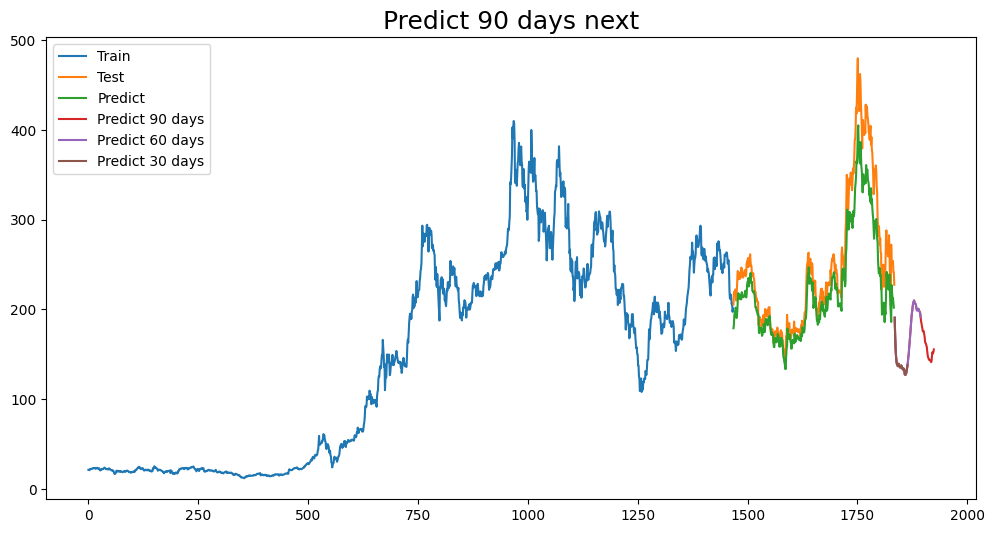
\includegraphics[width=0.8\textwidth]{resnet_predictions.png}
%     \caption{Actual and predicted stock prices using ResNet, including training data (blue), testing data (orange), test predictions (green), and forecasts for 30 (red), 60 (purple), and 90 days (brown).}
%     \label{fig:resnet_predictions}
% \end{figure}

% \begin{figure}[ht]
%     \centering
%     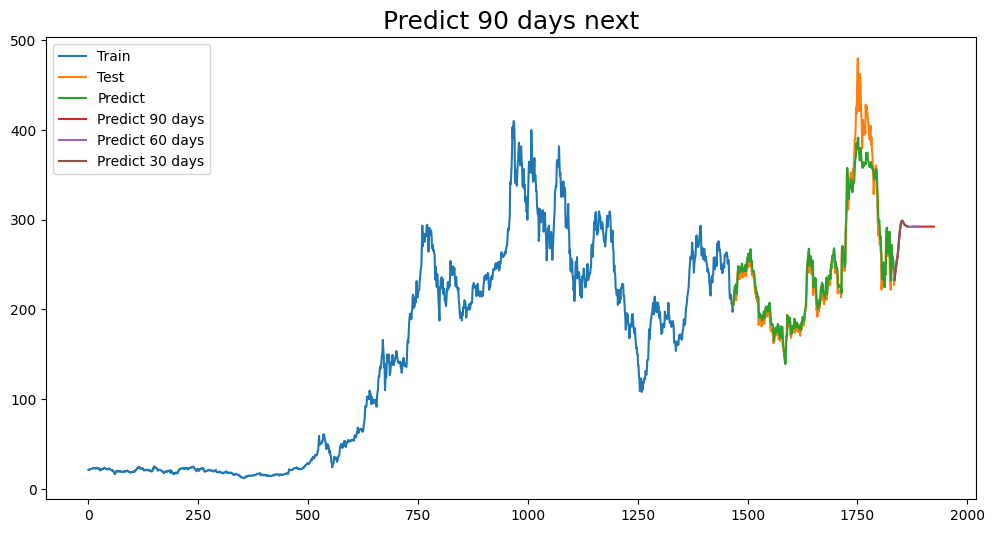
\includegraphics[width=0.8\textwidth]{resnetlstm_predictions.png}
%     \caption{Actual and predicted stock prices using ResNetLSTM, including training data (blue), testing data (orange), test predictions (green), and forecasts for 30 (brown), 60 (purple), and 90 days (red).}
%     \label{fig:resnetlstm_predictions}
% \end{figure}

\renewcommand{\refname}{References}
\bibliographystyle{plainnat}  % hoặc unsrtnat nếu bạn muốn theo thứ tự xuất hiện

\bibliography{references} % Link to references.bib
\end{document}